% LEXICAL STRESS ERRORS
%
% !TEX root = ../thesis-main.tex
%

\chapter{Lexical stress errors for French learners of German}

%\cleanchapterquote{You can’t do better design with a computer, but you can speed up your work enormously.}{Wim Crouwel}{(Graphic designer and typographer)}

%\blindtext

\section{Stress in German vs. French }
	\subsection{Comparative prosody}
	\subsection{Stress ``deafness'' in French}
	\subsection{Expected errors}
	
	
	
\section{Lexical stress errors in the IFCASL corpus} 

	\subsection{Data}

	\subsection{Annotation method}

	
		\begin{figure}
		\centering
		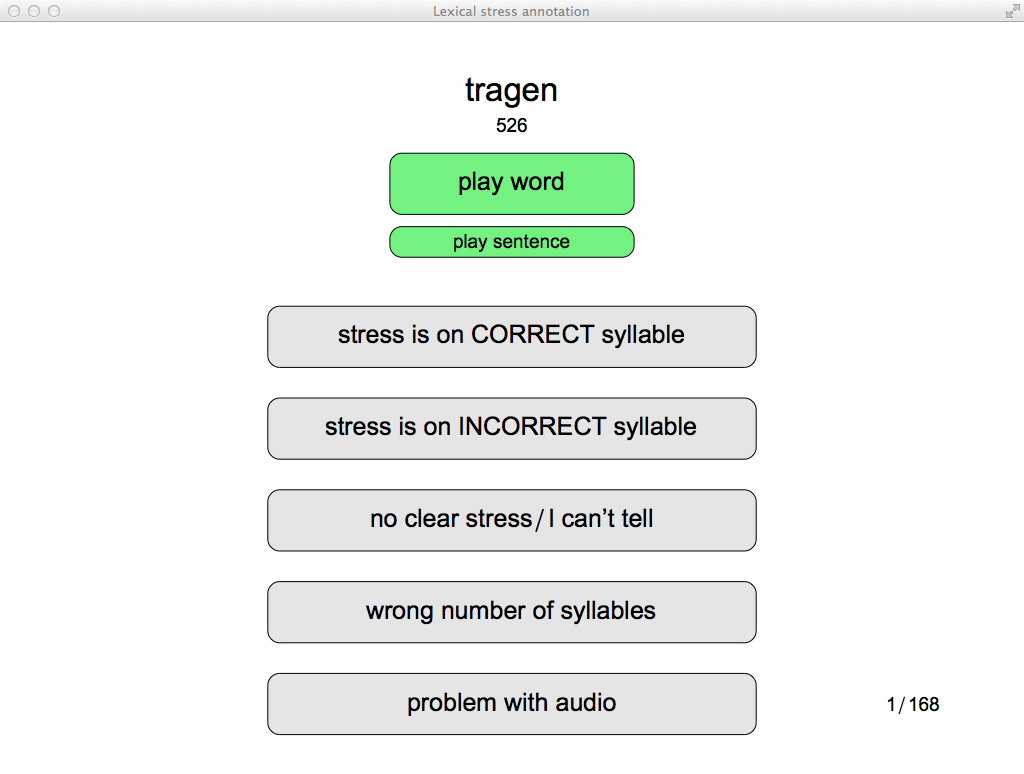
\includegraphics[width=\textwidth]{../img/screenshots/AnnotationTool}
		\caption{A screenshot of the graphical annotation tool scripted in Praat.  }
		\label{fig:annotationtool}
	\end{figure}
	
	The interface of the graphical annotation tool, scripted in Praat, is shown in \cref{fig:annotationtool}. At the top, a word's text is displayed, along with the ID number of the speaker whose utterance of that word will be annotated. The recording of the word, extracted from a longer sentence, is played automatically. The annotator may choose to play the word again, or play the entire sentence; either may be played as many times as the annotator wishes. Once the annotator has judged the accuracy of the lexical stress realization in this utterance, they log that judgment by clicking on one of the gray buttons. The annotator is then automatically advanced to the next utterance, with the counts in the lower right corner tracking their progress towards the total number of tokens to be annotated. 
	
	\subsection{Results}
		\subsubsection{Native vs. nonnative annotators}

		Of the \TODO annotators, \TODO were native German speakers, \TODO{2} were native speakers of English, and \TODO{one} annotator's first language was Hebrew. 

		In comparing the relative frequencies of the different response classes, we observe that the native and nonnative speakers judge utterances as having correct lexical stress with approximately the same frequency. However, nonnative speakers seem to choose the ``no clear stress/I can't tell'' somewhat more frequently than native speakers; this could be attributed to nonnative speakers being less confident about the how stress should be realized in German, resulting in less certainty about whether a given utterance is correct or not. \TODO{update/verify this paragraph}
		
		\subsubsection{Accuracy by L2 skill level}
		
		
		
		\subsubsection{Accuracy by word type}

%\section{Frequency of production}
%\section{Impact on Intelligibility}
%\section{Automatic detection}